\documentclass[a4paper,11pt,openright]{book}

\usepackage[utf8]{inputenc}
\usepackage{csquotes}
\usepackage[top=2cm,bottom=2cm,left=2cm,right=2cm]{geometry}
\usepackage[pdftex]{graphicx} %per poter inserire le figure
\usepackage{amssymb,amsmath,amsthm,amsfonts}
\usepackage{bm}
\usepackage{xcolor}
\usepackage{xspace}
\usepackage{tabularx}
\usepackage{indentfirst}
\usepackage{subfigure}
\usepackage{graphicx}
\usepackage[small]{caption}
\usepackage{eucal}
\usepackage{eso-pic}
\usepackage{url}
\usepackage{booktabs}
\usepackage{afterpage}
\usepackage{parskip}
\usepackage{listings}
\usepackage{fancyhdr}
\usepackage{textcomp}
\usepackage{multirow}
\usepackage{comment}
\usepackage{wrapfig}
\usepackage[italian]{babel}   %per riuscire a scrivere gli accenti
\usepackage{setspace}
\usepackage{hyperref}
\usepackage{enumitem}
\setlist[itemize]{noitemsep}
\setlist[enumerate]{noitemsep}
\usepackage{mdframed}
\newmdenv[
  topline=false,
  bottomline=false,
  skipabove=\topsep,
  skipbelow=\topsep
]{siderules}
\usepackage{float}
\usepackage{longtable}

\usepackage[
backend=biber,
bibstyle=authoryear,
citestyle=authoryear,
sorting=nyt
]{biblatex}


\usepackage{xcolor}
\setlength{\fboxrule}{0.1pt} % Thickness of the frame
\setlength{\fboxsep}{2pt}  % Space between the frame and the image
\makeatletter
\newrobustcmd*{\parentexttrack}[1]{%
  \begingroup
  \blx@blxinit
  \blx@setsfcodes
  \blx@bibopenparen#1\blx@bibcloseparen
  \endgroup}
\AtEveryCite{%
  \let\parentext=\parentexttrack%
  \let\bibopenparen=\bibopenbracket%
  \let\bibcloseparen=\bibclosebracket}
\makeatother

%%%%%%%%%%%%%%% head and foot notes %%%%%%%%%%%%%%%%%%%%%%%%%%%%%%%%%%%%%%%
\pagestyle{fancy}
\fancyhf{} % Clear header and footer fields
% Remove the header and footer lines
\renewcommand{\headrulewidth}{0pt}
%\renewcommand{\footrulewidth}{0pt}
% Redefine the fancy style for chapters
\fancypagestyle{plain}{
  \fancyhf{} % Clear header and footer fields
}
% Set the page number to be displayed at the bottom right
\rfoot{\thepage}

% Set numbering for chapter head pages
\fancypagestyle{plain}{% % <-- this is new
  \fancyhf{} 
  \fancyfoot[LE,RO]{\thepage} % same placement as with page style "fancy"
  \renewcommand{\headrulewidth}{0pt}}

%%%%%%%%%%%%%%%%%%%%%%%%%% chapter head style %%%%%%%%%%%%%%%%%%%%%%%%%%%%%%%%%%%%%
\usepackage[T1]{fontenc}
\usepackage{titlesec}
\newcommand{\chapnumfont}{%     % define font for chapter number
  \usefont{T1}{pnc}{b}{n}%      % choose New Chancery, bold, normal shape
  \fontsize{70}{100}%          % font size 100pt, baselineskip 100pt
  \selectfont%                  % activate font
}
\colorlet{chapnumcol}{gray!75}  % color for chapter number

\titleformat{\chapter}[display]
{\filleft} % add \bfseries to chage font of chapter title to bold
{\filleft\chapnumfont\textcolor{chapnumcol}{\thechapter}} 
{-24pt}
{\fontsize{24}{24}\selectfont}
\titlespacing*{\chapter}{0pt}{0pt}{20pt} % 
% Customize table of contents 
\usepackage{titletoc}

\titlecontents{chapter}[1.5em]
{\addvspace{1em}\bfseries}
{\contentslabel{1.5em}}
{}{\titlerule*[0pt]{.}\contentspage}

\titlecontents{section}[3.em] %adjust indendation
{\normalfont}
{\contentslabel{1.5em}}
{}{\titlerule*[8pt]{.}\contentspage}

\titlecontents{subsection}[5.3em]
{\normalfont}
{\contentslabel{2.3em}}
{}{\titlerule*[8pt]{.}\contentspage}


%TEOREMI
\usepackage{amsthm}
\newtheoremstyle{a capo}% nome dello stile
  {\topsep}% spazio sopra
  {\topsep}% spazio sotto
  {\itshape}% font del corpo
  {}% indentazione del primo paragrafo
  {\bfseries}% font dell'intestazione
  {}% punteggiatura dopo l'intestazione
  {\newline}% spazio dopo l'intestazione
  {\thmname{#1}\thmnumber{ #2}\thmnote{ (#3)}}% formato dell'intestazione
 \newtheoremstyle{due punti}% nome dello stile
  {\topsep}% spazio sopra
  {\topsep}% spazio sotto
  {\itshape}% font del corpo
  {}% indentazione del primo paragrafo
  {\bfseries}% font dell'intestazione
  {:}% punteggiatura dopo l'intestazione
  { }% spazio dopo l'intestazione
  {\thmname{#1}\thmnumber{ #2}\thmnote{ (#3)}}% formato dell'intestazione


\newtheorem{df}{Definition}
\newtheorem{pr}{Principle}
\newtheorem{pro}{Proposition}
\newtheorem{cor}{Corollary}
\newtheorem{teo}{Theorem}
\newtheorem{lemma}{Lemma}

\counterwithin{df}{subsection}
\counterwithin*{pr}{subsection}
\counterwithin{pro}{subsection}
\counterwithin{cor}{subsection}
\counterwithin{teo}{subsection}

\addbibresource{bibliography.bib}


\begin{document}
\frontmatter
\begin{titlepage}
\vspace{5mm}
\begin{center}
{{\huge{\textsc{\bf UNIVERSIT\`A DEGLI STUDI DI PADOVA}}}\\}
\vspace{5mm}
{\Large{\bf Dipartimento di Fisica e Astronomia ``Galileo Galilei''}} \\
\vspace{5mm}
\begin{spacing}{3}
{\LARGE \textbf{Applicazione della teoria del trasporto ottimo alla modellizzazione ecologica e per la inferenza della rete di interazione tra specie.}}\\
\end{spacing}
\vspace{8mm}
\end{center}

\vspace{10mm}
\begin{spacing}{2}
\begin{tabular}{ l  c  c c c cc c c c c c c c c c c  l }
{\Large{ Responsabile scientifico}} &&&&&&&&&&&&&&&&& {\Large{Studentessa}}\\
{\Large{\bf Samir Simon Suweis}} &&&&&&&&&&&&&&&&& {\Large{\bf Miriam Zara}}\\
{\Large{ Corresponsabile scientifico}} &&&&&&&&&&&&&&&&& \\
{\Large{\bf Sandro Azaele}} &&&&&&&&&&&&&&&&& \\

\end{tabular}
\end{spacing}
\vspace{10mm}

\begin{center}
{\Large \today }
\end{center}
\vspace*{5mm}
Abstract:


\end{titlepage}
\clearpage{\pagestyle{empty}\cleardoublepage}
\tableofcontents
\mainmatter
\chapter{Mathematical Modeling Basics}

\section{A general class of models}
The class of models we will be concerned about takes this form;
\begin{equation}
    \dot{x}_i(t) = x_i(t)\cdot f_i[x(t)]
\end{equation}
The reason behind the choice to factor out $x_i$ is to highlight that in this class of models invasion of the ecosystem is not allowed: if a species is not present at time $t=0$, it cannot enter the ecosystem at later times. 
\section{Types of ecological interactions, with some real world examples}
\begin{figure}[H]
\centering
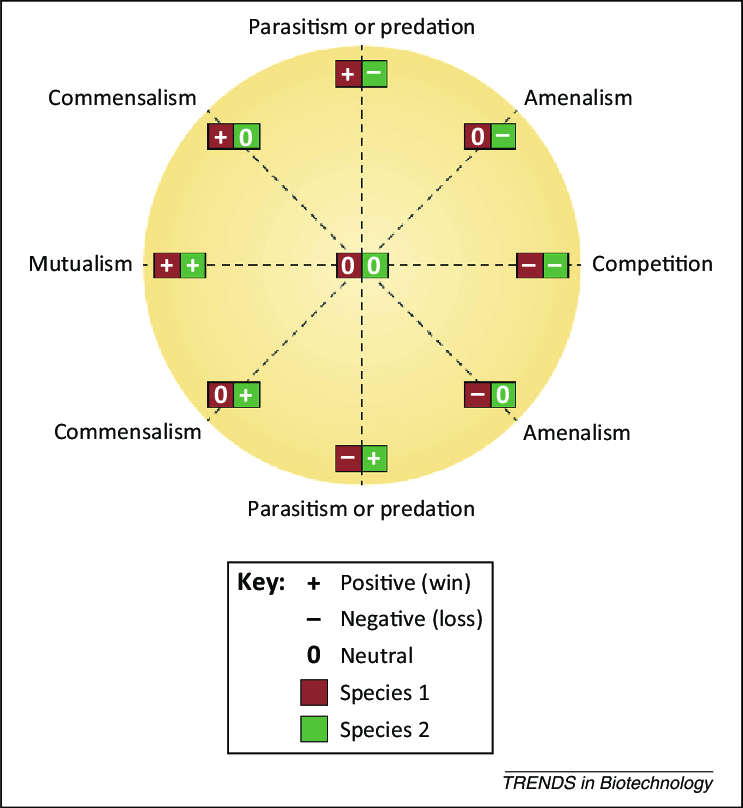
\includegraphics[width=0.4\linewidth]{figures/chapter_1/Ecological-interactions-among-microbial-species-For-any-two-interacting-species-there.png}
    \caption{The six types of ecological interactions}
    \label{fig:eco_interactions}
\end{figure}
\begin{itemize}
    \item Syntrophy: is a specific type of mutualistic (+ +) relationship where two or more species cooperate to degrade a substrate that neither species can break down alone. The metabolic products of one organism are essential for the other organism to thrive, and vice versa. Syntrophy often occurs when the degradation of a compound requires a sequential or coupled process that depends on the interaction of different species.
	The classic example is methanogenic syntrophy in anaerobic environments: certain bacteria break down complex organic matter into simpler compounds like hydrogen ($H_2$) and acetate. However, high levels of $H_2$ can inhibit their activity. Methanogens (archaea) consume $H_2$, converting it into methane ($CH_4$), which lowers the $H_2$ concentration, allowing the bacteria to continue their breakdown process. Without the methanogens, the bacteria couldn’t degrade the organic matter efficiently. This makes the interaction beneficial for both sides (++). 
	\item Cross-Feeding: is a broader term that refers to any process where one organism consumes the metabolic by-products of another organism, regardless of whether this interaction is obligatory for either species. It can be mutualistic (+ +), but it can also be commensal (+ 0), where one species benefits without affecting the other. A well-known example is lactate cross-feeding in the human gut microbiome: \textit{Bifidobacteria} ferment dietary fibers into lactate. Certain butyrate-producing bacteria, such as \textit{Eubacterium hallii}, consume lactate and convert it into butyrate, a short-chain fatty acid beneficial for gut health. This relationship benefits the butyrate producers but is not strictly required for the bifidobacteria.
\end{itemize}
\section{Ecological interactions can be context- dependent}
There is experimental evidence that the type  (the sign) and the strength of ecological interactions between species can change, depending on biotic and abiotic \footnote{Biotic means living and abiotic means non - living. For example, considering the microbiota ecosystem, some abiotic factors include the host's diet, the host's immune system response, the body temperature. Biotic factors, instead, include for example the metabolic products of the species and the species population densities.} factors in the environment. This fact is commonly referred to as \textit{context-dependency}. That is, there are situations where the type of interaction (mutualism, commensalism, competition etc..) cannot be assumed as fixed, and species can behave in different ways with respect to each other if conditions change in the environment, for example switching from midly competing to strongly competing, or even from competing to mutualistic and so on.

In mathematical terms, this means that the sign pattern of the Jacobian matrix at equilibrium (the community matrix) may change across the different steady (or equilibrium) states of the system. The community matrix details the effect of increasing the density of one species on any other species around the equilibrium point.


\begin{center}
\begin{align}
    \dot{x}_i(t) = x_i(t)\cdot f_i[x(t)] \\
    \overline{x}\,\, \text{steady state}\,\, J(\overline{x})_{i,\,j} = \frac{\partial f_i}{\partial_j} \,\, \text{community matrix at equilibrium}\,\, \overline{x}
\end{align}
\end{center}
This fact adds complexity to the task of building models for species evolution. 

\textbf{Key Idea}
   \textit{Species populations across different environmental conditions or community memberships generate distinct interspecies interaction networks, the comparison of which may provide an idea of how interactions are modulated by the impact of abiotic and biotic factors (es: how will the climate change affect the ecosystems?)} 

The generalized Lokta Volterra model does not account for context- dependency of interactions. Instead, one class of models that can account for context-dependency is the \textbf{Consumer - Resource models (CRM)} class. A paradigmatic CRM is the Mac Arthur's consumer-resource model (MCRM).

A general consumer-resource model consists of \( M \) resources whose abundances are \( R_1, \ldots, R_M \) and \( S \) consumer species whose populations are \( N_1, \ldots, N_S \). A general consumer-resource model is described by the system of coupled ordinary differential equations,

\[
\frac{dN_i}{dt} = N_i g_i(R_1, \ldots, R_M), \quad i = 1, \ldots, S,
\]

\[
\frac{dR_\alpha}{dt} = f_\alpha(R_1, \ldots, R_M, N_1, \ldots, N_S), \quad \alpha = 1, \ldots, M,
\]

where \( g_i \), depending only on resource abundances, is the per-capita growth rate of species \( i \), and \( f_\alpha \) is the growth rate of resource \( \alpha \). An essential feature of CRMs is that species growth rates and populations are mediated through resources and there are no explicit species-species interactions. Through resource interactions, there are emergent inter-species interactions.(source: Wikipedia Eng Consumer-Resource Models).




\subsection{Some real world examples of context - dependency}
Some of the most common factors that may shift the interaction type and strength are resource availability and population density.
\begin{itemize}
    \item Plant-fungi relationships (mutualism to commensalism to parasitism):

Many plants form mycorrhizal associations with fungi, where fungi enhance nutrient uptake for the plant (a mutualistic relationship). However, in nutrient-rich soils, allocating resources to the fungi can become disadvantageous for the plant. Thus, the fungi effectively becomes a parasite. \parencite{mycorrhizal}.

    \item Quorum sensing virulence expression:\\
    Bacteria often communicate using quorum sensing, a mechanism where they release signaling molecules into their environment to detect population density.  Many pathogenic bacteria are harmless when their population densities are low. At low densities, they might exist in a commensal relationship with the host or other bacteria. However, when their density surpasses a certain threshold (as detected via quorum sensing), they might collectively express virulence factors, turning from harmless commensals into aggressive pathogens.
    \item 
    Glucose alters the symbiotic relationships between the host and the gut microbiota. \\ For instance, glucose metabolism by Escherichia coli increases the production of organic acids,
    which lowers intestinal pH resulting in reduced survival of Vibrio cholerae in the
    host. This represents a mutualistic interaction between host glucose and a commensal
    (E. coli) to combat a potential pathogen (V.
    cholerae). Also, high glucose availability in the
    jejunum, cecum, and colon can result in
    increased glucose metabolism by certain
    pathogenic bacteria. This increased bacterial
    glucose flux can reduce virulence and tip the
    balance from parasitism to commensalism. 
    \parencite{doi:10.1152/ajpendo.00485.2019}.
\end{itemize}



\subsection{Community matrix in the gLV model has fixed sign pattern for feasible equilibria.}
The classic generalized lokta volterra is the simplest possible model of species interactions. It assumes fixed sign and strength of interactions. As a consequence of this assumption, \textit{the sign pattern of the community matrix is fixed across all feasible equilibria} \parencite{Allesina_Brasil}.

Generalized deterministic Lokta Volterra
\begin{equation}
    \centering
     \dot{x}_i(t) = x_i(t)\cdot \left[ r_i\, + \sum_j\, a_{i,\,j}\, x_j \right] \label{eq:gLV}
\end{equation}
where the $r_i$ are the intrinsic growth rates, $a_{i,\,j }$ are the interaction terms. Usually, growth rates are taken as negative to account for a limited carrying capacity of the environment (logistic growth).
In compact matrix form:
\begin{equation}
    \centering
    \dot{x} = \text{diag}(x)\,\cdot \left[r + A\cdot x\right] = f(x)
\end{equation}

Then lets compute the entries of the community matrix at the feasible equilibrium $\overline{x}$:
\begin{align}
    \begin{cases}
    \frac{\partial f_i}{\partial x_j} = a_{i,\,j}\, \overline{x}_i \quad i\neq j \\
    \frac{\partial f_i}{\partial x_j} = [r + A\overline{x}]_i+ a_{i,\,i}\overline{x}_i \quad i= j \\
    \end{cases}
\end{align}:
A \textit{feasible equilibrium}, by definition, is an equilibrium in the positive open subset of $\mathbb{R}^n$, $\mathbb{R}^n_{+} = \{x | x_i > 0\, \forall i\}$, that is an equilibrium where all the species coexist with positive abundances. Since in a feasible equilibrium $\text{diag}(\overline{x})$ has all positive entries, $\overline{x}$ must satisfy
\begin{equation}
\begin{cases}
r + A \overline{x} = 0 \\
\overline{x}_i > 0\quad \forall i \\
\end{cases}
\end{equation}
Solutions to the first equation depends on $rk[A|r]$.  Let us suppose solutions exist ($rk[A|r] = rk[A]$). The community matrix at the feasible equilibrium satisfies
\begin{equation}
    J_{i,\,j} = a_{i,\,j}\,\overline{x}_i \quad \forall x_{i,\,j}
\end{equation}
In particular, in case multiple feasible equilibria do exist ($rk[A]< n$ and $rk[A|r] = rk[A]$), the sign patter of their community matrix is always the same and is equal to the sign pattern of the interaction matrix $A$.

\chapter{Analysis of the MICEGUT dataset}
\section{Dataset Description}
\textcolor{red}{to be completed}
\begin{figure}[H]
\centering
\fcolorbox{black}{white}{
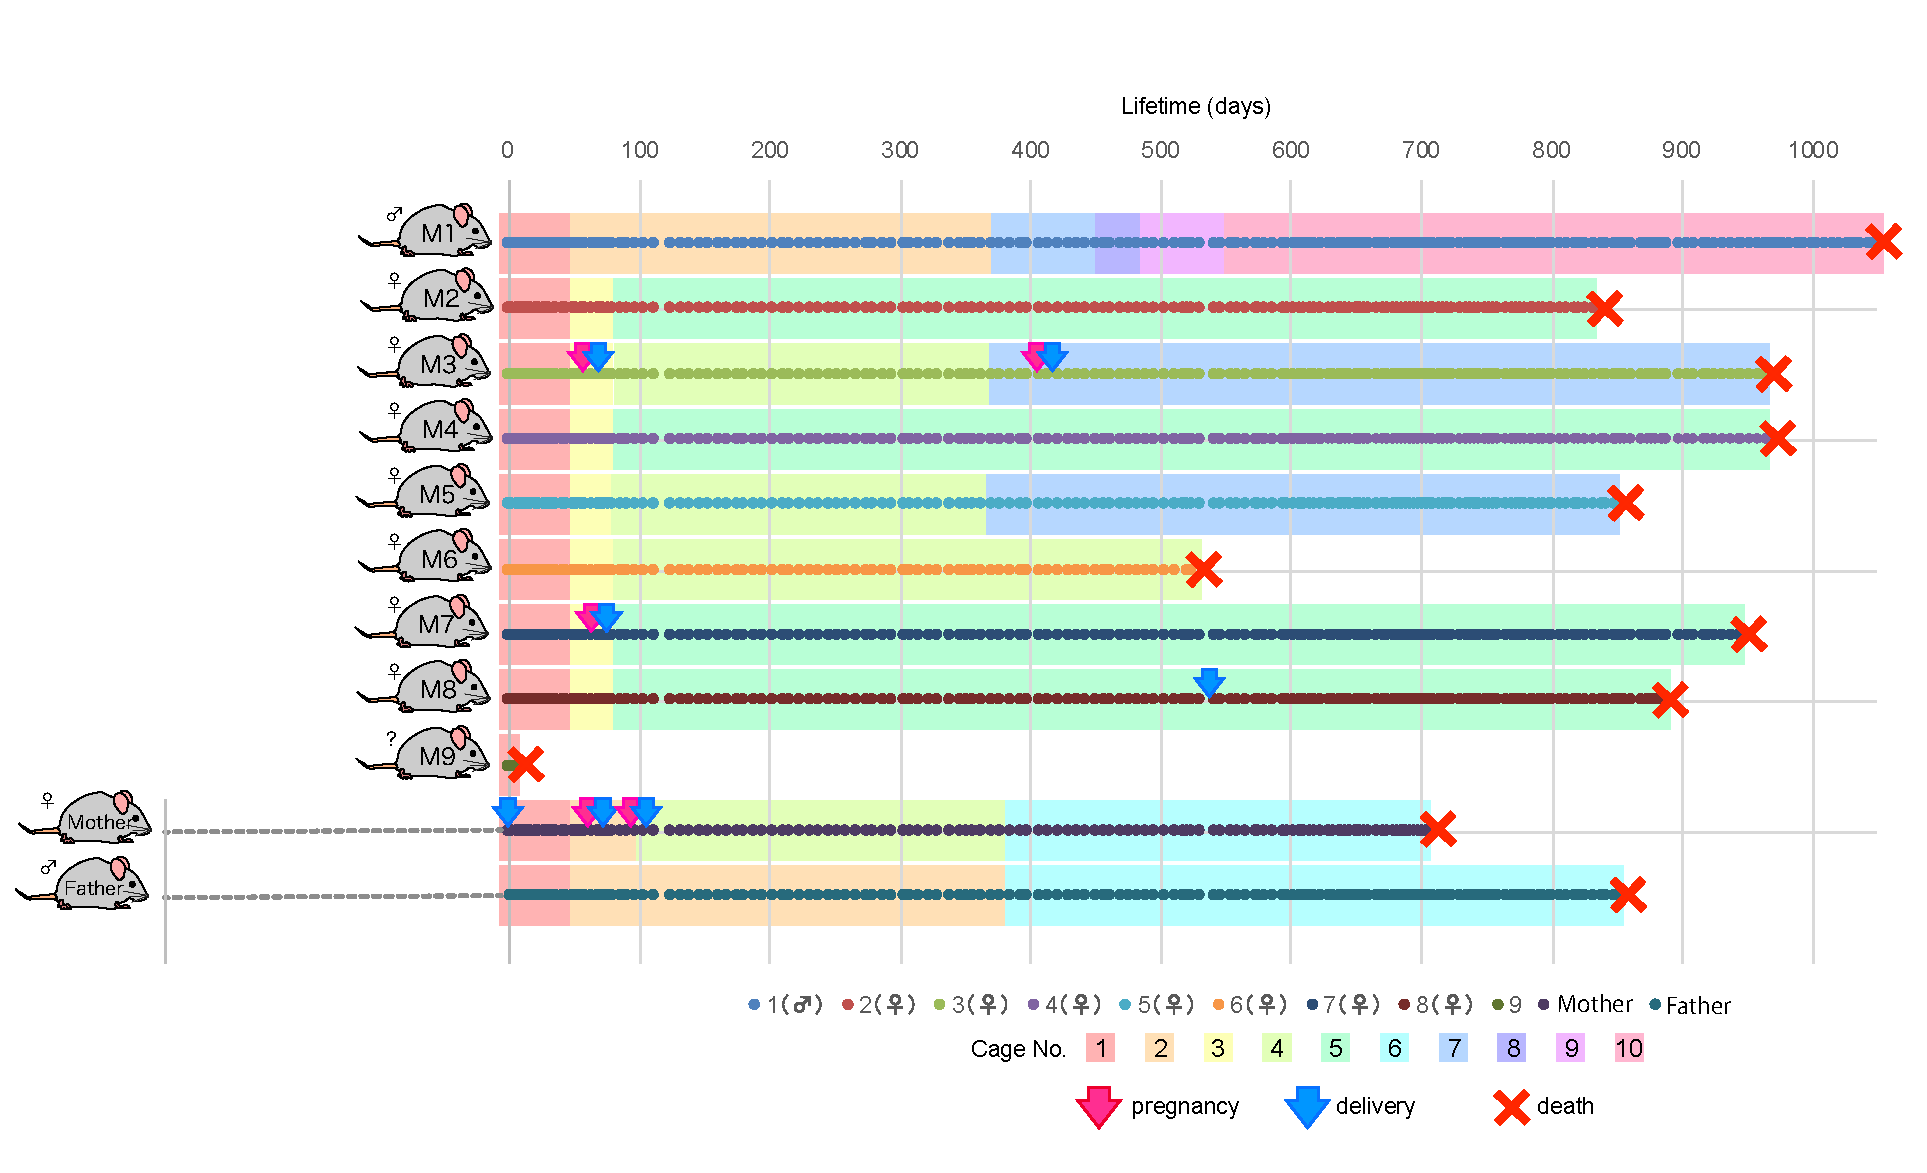
\includegraphics[width = 0.6\linewidth]{figures/chapter_2/fig_data.pdf}
}
\caption{}
\end{figure}

\newpage

\section{Summary Statistics}
\subsection{Rank- Abundance distributions}

\begin{figure}[H]
    \centering
    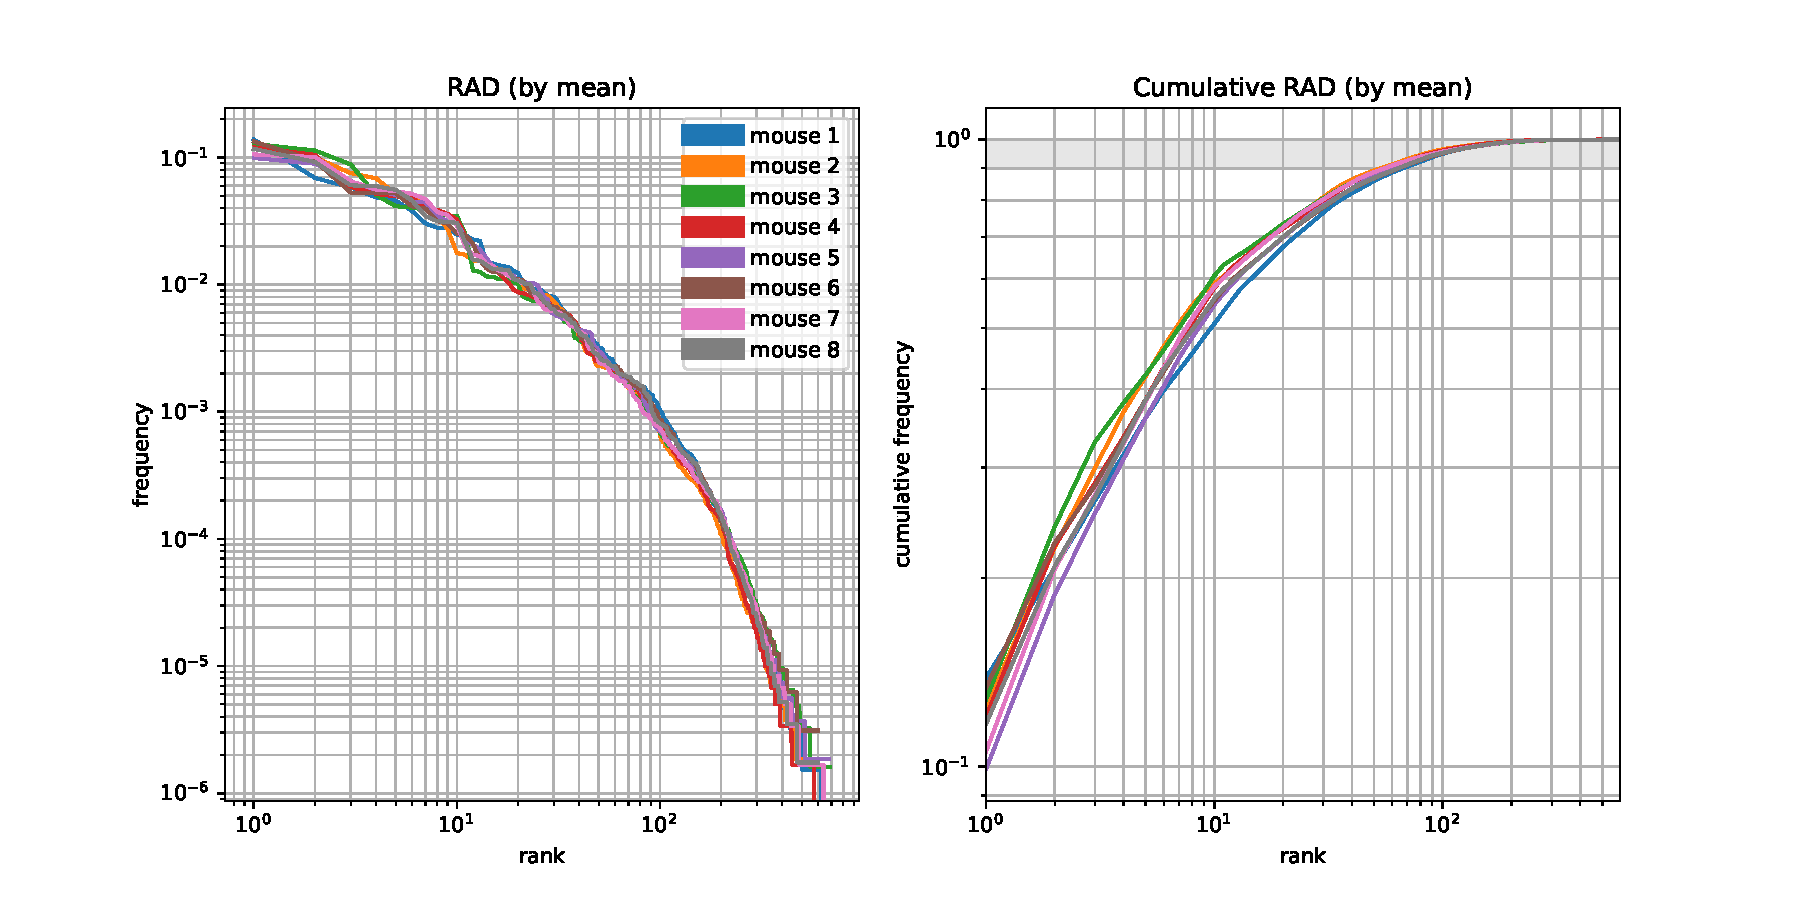
\includegraphics[width=\linewidth]{figures/chapter_2/RAD_mean.pdf}
    \caption{Caption}
    \label{fig:enter-label}
\end{figure}
\subsection{Sample composition across subjects}

\begin{figure}[H]
\centering
\subfigure[]{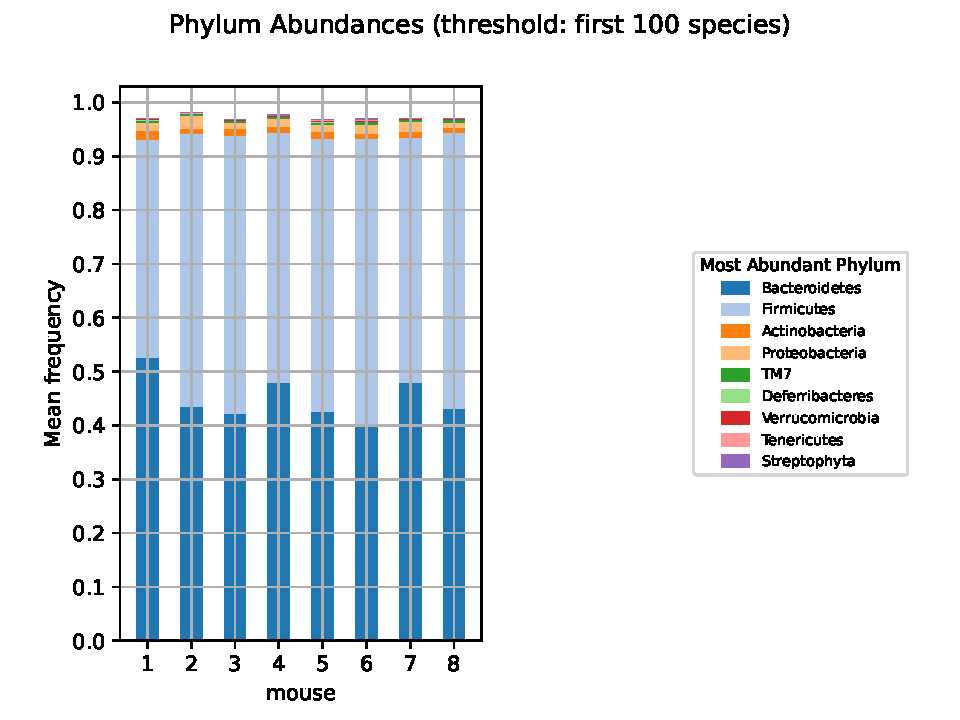
\includegraphics[width=0.48\linewidth]{figures/chapter_2/Phylum_stacked_first_100.pdf}}
\hfill
\subfigure[]{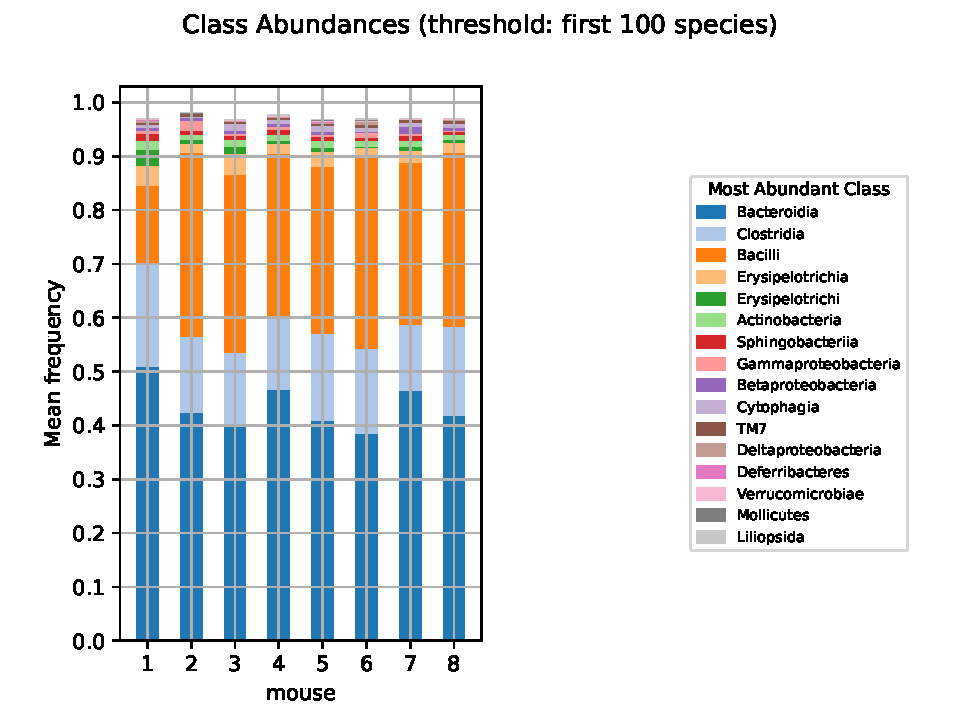
\includegraphics[width=0.48\linewidth]{figures/chapter_2/Class_stacked_first_100.pdf}}
\vspace*{1cm}
\subfigure[]{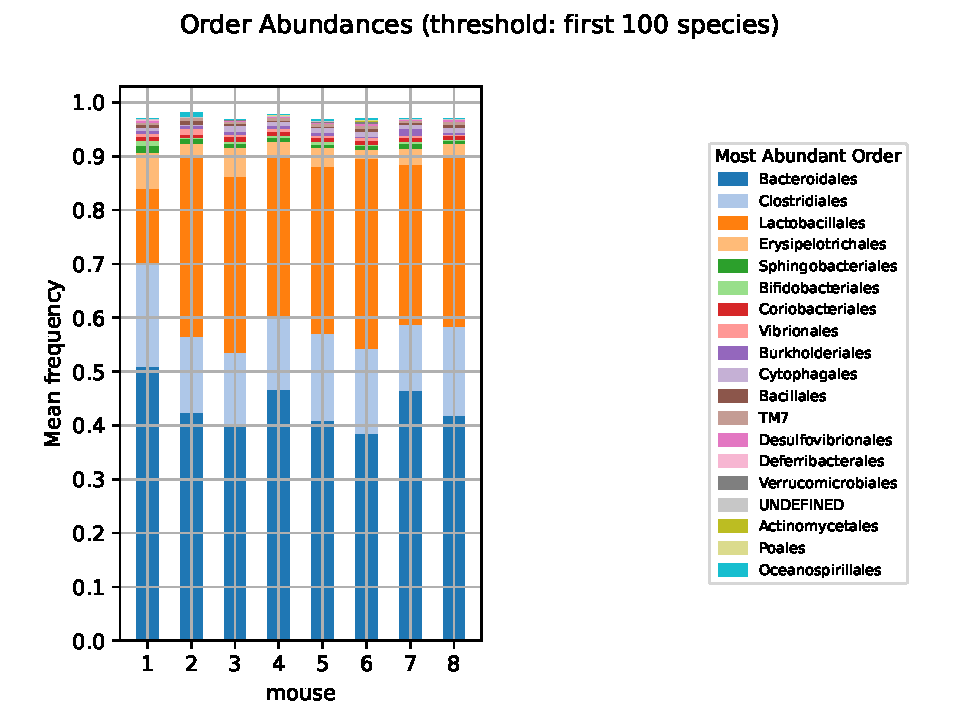
\includegraphics[width=0.48\linewidth]{figures/chapter_2/Order_stacked_first_100.pdf}}
\hfill
\subfigure[]{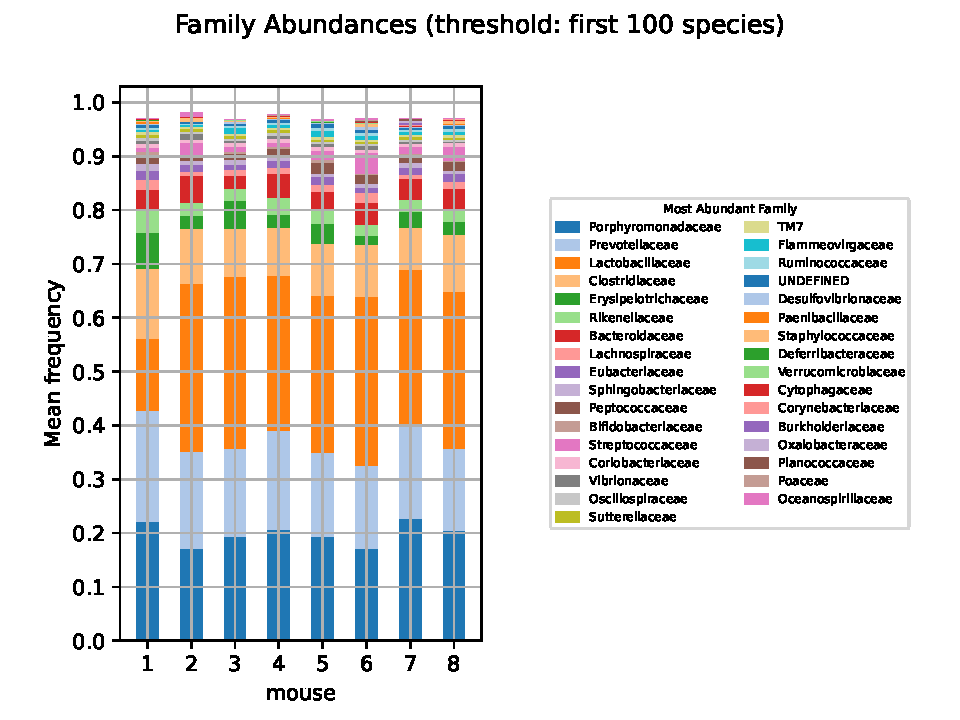
\includegraphics[width=0.48\linewidth]{figures/chapter_2/Family_stacked_first_100.pdf}}
\vspace*{1cm}
\caption{Caption}
\end{figure}

\begin{figure}[H]
    \centering
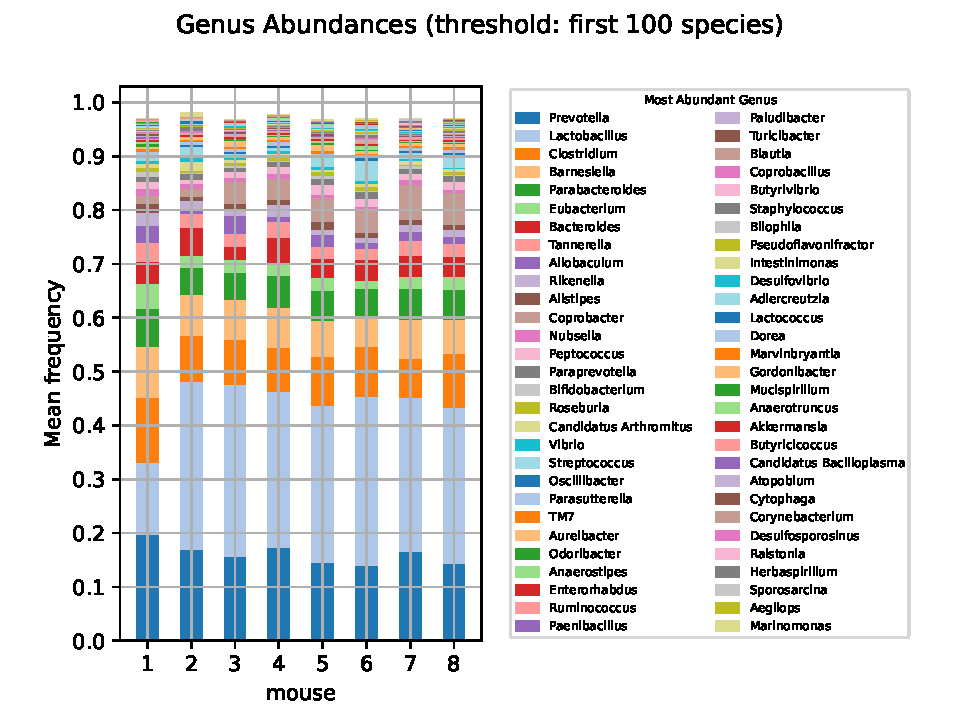
\includegraphics[width=0.9\linewidth]{figures/chapter_2/Genus_stacked_first_100.pdf}

    \label{fig:enter-label}
\end{figure}

\begin{figure}[H]\ContinuedFloat
    \centering
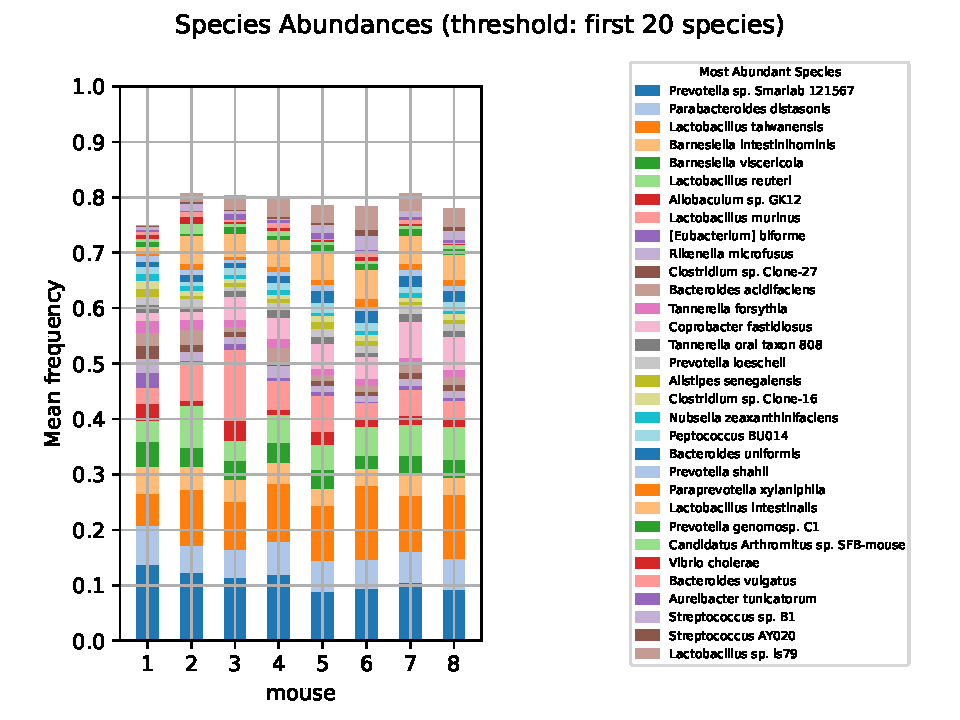
\includegraphics[width=0.9\linewidth]{figures/chapter_2/Species_stacked_first_20.pdf}
    \caption{Taxonomic ranks from bottom to top are:
Species $\subset$ Genus $\subset$ Family $\subset$ Order $\subset$ Class $\subset$ Phylum.}
    \label{fig:enter-label}
\end{figure}

\newpage
\section{Species abundance summary data \textcolor{red}{TO BE COMPLETED}.}



\textcolor{red}{MISSING: Estimation of inter-class and intra-class variance using Linear Mixed Models}
\begin{figure}[H]
    \centering
    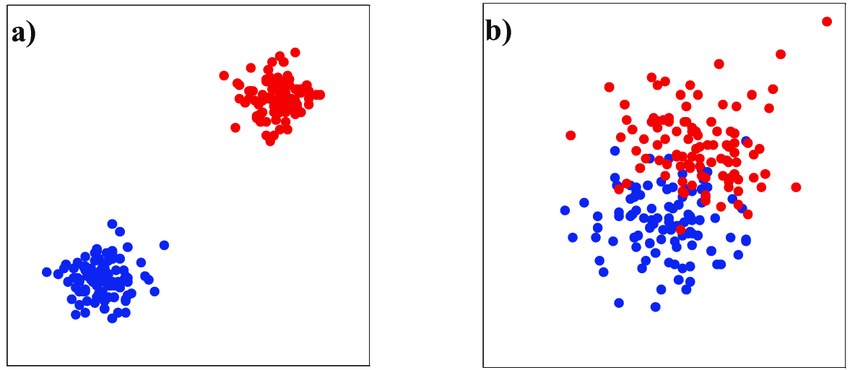
\includegraphics[width=0.5\linewidth]{figures/chapter_2/temp.png}
    \caption{\textcolor{red}{As a reminder.} Inter-class and Intra-class variances concept. a) Low intra-class variance and high inter-class variance: compact well separated clusters. b) High intra-class variance and low inter-class variance: wide clusters without a clear frontier. }
    \label{fig:temp}
\end{figure}

\begin{center}
\begin{longtable}{|l|l|l|l|}
\caption{The table shows the median counts and the mean counts for $136$ species, taken as the union of the $100$ most abundant species by median counts in all mice. The mean counts entry in the table refers to the mean of the mean counts in each mouse.} \label{tab:species_counts} 


\\ \hline \multicolumn{1}{|c|}{\textbf{Rank}} & \multicolumn{1}{c|}{\textbf{Species}} & \multicolumn{1}{c|}{\textbf{Mean counts}} &
\multicolumn{1}{c|}{\textbf{Median counts}}\\
\hline \endfirsthead

\multicolumn{4}{c}% 
{{\tablename\ \thetable{} -- continued from previous page}} \\
\hline \multicolumn{1}{|c|}{\textbf{Rank}} & \multicolumn{1}{c|}{\textbf{Species}} & \multicolumn{1}{c|}{\textbf{Mean counts}} &
\multicolumn{1}{c|}{\textbf{Median counts}}\\
\hline 
\endhead

 \hline 
 \multicolumn{4}{|r|}{Continued on next page}
 \\
 \hline
\endfoot


\hline \hline
\endlastfoot
$1$ & Prevotella sp. Smarlab 121567 & $328.61$ & $320.23$ \\
$2$ & Lactobacillus taiwanensis & $300.42$ & $263.12$ \\
$3$ & Lactobacillus murinus & $170.44$ & $73.31$ \\
$4$ & Parabacteroides distasonis & $167.60$ & $171.12$ \\
$5$ & Lactobacillus reuteri & $153.84$ & $130.00$ \\
$6$ & Lactobacillus intestinalis & $131.43$ & $104.62$ \\
$7$ & Coprobacter fastidiosus & $119.23$ & $93.81$ \\
$8$ & Barnesiella intestinihominis & $111.12$ & $111.52$ \\
$9$ & Barnesiella viscericola & $104.04$ & $103.69$ \\
$10$ & Lactobacillus sp. ls79 & $77.73$ & $61.69$ \\
$11$ & Allobaculum sp. GK12 & $56.04$ & $15.19$ \\
$12$ & Bacteroides acidifaciens & $51.08$ & $32.25$ \\
$13$ & Bacteroides uniformis & $47.93$ & $33.31$ \\
$14$ & Rikenella microfusus & $44.60$ & $37.44$ \\
$15$ & Tannerella forsythia & $44.11$ & $42.38$ \\
$16$ & Peptococcus BU014 & $39.93$ & $27.56$ \\
$17$ & Prevotella loescheii & $39.85$ & $32.38$ \\
$18$ & Tannerella oral taxon 808 & $34.71$ & $30.81$ \\
$19$ & Clostridium sp. Clone-27 & $34.23$ & $13.56$ \\
$20$ & Streptococcus sp. B1 & $33.42$ & $0.00$ \\
$21$ & Paraprevotella xylaniphila & $29.45$ & $19.69$ \\
$22$ & Prevotella genomosp. C1 & $28.07$ & $26.27$ \\
$23$ & Clostridium sp. Clone-16 & $27.81$ & $14.81$ \\
$24$ & [Eubacterium] biforme & $26.30$ & $0.38$ \\
$25$ & Prevotella shahii & $25.90$ & $21.19$ \\
$26$ & Alistipes senegalensis & $25.76$ & $15.12$ \\
$27$ & Nubsella zeaxanthinifaciens & $24.62$ & $23.25$ \\
$28$ & Clostridium sp. Clone-9 & $23.00$ & $11.88$ \\
$29$ & Candidatus Arthromitus sp. SFB-mouse & $22.84$ & $9.00$ \\
$30$ & Prevotella sp. oral taxon 317 & $21.48$ & $20.29$ \\
$31$ & Aureibacter tunicatorum & $19.81$ & $16.12$ \\
$32$ & Clostridium hathewayi & $18.46$ & $10.56$ \\
$33$ & Candidatus Prevotella conceptionensis & $17.26$ & $16.06$ \\
$34$ & Vibrio cholerae & $16.72$ & $0.00$ \\
$35$ & Bacteroides vulgatus & $16.58$ & $9.31$ \\
$36$ & Clostridium sp. ID4 & $15.93$ & $6.06$ \\
$37$ & Parasutterella excrementihominis & $14.24$ & $11.88$ \\
$38$ & TM7 oral taxon 351 & $13.97$ & $12.25$ \\
$39$ & Streptococcus AY020 & $13.06$ & $0.62$ \\
$40$ & Eubacterium sp. F1 & $12.94$ & $7.81$ \\
$41$ & Clostridium sp. ASF502 & $12.62$ & $5.25$ \\
$42$ & Bifidobacterium pseudolongum & $12.18$ & $0.00$ \\
$43$ & Clostridium disporicum & $11.41$ & $2.62$ \\
$44$ & Eubacterium coprostanoligenes & $10.21$ & $6.25$ \\
$45$ & Enterorhabdus caecimuris & $9.82$ & $8.12$ \\
$46$ & [Eubacterium] cylindroides & $9.21$ & $3.75$ \\
$47$ & Eubacterium ventriosum & $8.86$ & $4.69$ \\
$48$ & Staphylococcus aureus & $8.75$ & $0.00$ \\
$49$ & Clostridium indolis & $8.42$ & $3.50$ \\
$50$ & Odoribacter splanchnicus & $8.23$ & $5.00$ \\
$51$ & Prevotella oulorum & $8.11$ & $7.85$ \\
$52$ & Clostridium fusiformis & $8.06$ & $5.00$ \\
$53$ & Clostridium sp. 6-44 & $8.02$ & $5.25$ \\
$54$ & Pseudoflavonifractor capillosus & $7.82$ & $5.94$ \\
$55$ & Prevotella oris & $7.77$ & $7.49$ \\
$56$ & Clostridium sp. Culture-27 & $7.60$ & $3.62$ \\
$57$ & Roseburia sp. 1120 & $7.45$ & $0.25$ \\
$58$ & Oscillibacter valericigenes & $7.27$ & $5.06$ \\
$59$ & Clostridium sp. CRIB & $6.88$ & $2.12$ \\
$60$ & Prevotella IK062 & $6.49$ & $0.38$ \\
$61$ & Clostridium aminophilum & $6.45$ & $2.69$ \\
$62$ & Lactococcus garvieae & $6.09$ & $2.25$ \\
$63$ & Desulfovibrio desulfuricans & $5.88$ & $2.31$ \\
$64$ & Anaerostipes caccae & $5.84$ & $0.62$ \\
$65$ & Ruminococcus lactaris & $5.78$ & $2.88$ \\
$66$ & Paludibacter propionicigenes & $5.62$ & $5.25$ \\
$67$ & Oscillibacter sp. G2 & $5.60$ & $3.38$ \\
$68$ & Clostridium sp. Clone-46 & $5.46$ & $1.62$ \\
$69$ & Adlercreutzia equolifaciens & $5.38$ & $4.25$ \\
$70$ & Clostridium sp. Culture-46 & $5.31$ & $2.38$ \\
$71$ & Clostridium scindens & $5.24$ & $2.25$ \\
$72$ & Clostridium sp. Culture-57 & $5.18$ & $0.81$ \\
$73$ & Dorea longicatena & $5.18$ & $2.56$ \\
$74$ & Alistipes putredinis & $5.12$ & $4.25$ \\
$75$ & Clostridium phytofermentans & $4.96$ & $0.88$ \\
$76$ & Turicibacter sp. LA62 & $4.89$ & $0.62$ \\
$77$ & Clostridium sp. Clone-26 & $4.67$ & $1.75$ \\
$78$ & Clostridium sp. 619 & $4.51$ & $3.25$ \\
$79$ & Clostridium sp. SY8519 & $4.38$ & $1.50$ \\
$80$ & Eubacterium plexicaudatum & $4.33$ & $1.00$ \\
$81$ & Roseburia hominis & $4.28$ & $2.25$ \\
$82$ & Clostridium sp. Culture-23 & $4.26$ & $2.06$ \\
$83$ & Clostridium sp. Clone-44 & $4.24$ & $1.75$ \\
$84$ & Intestinimonas butyriciproducens & $4.14$ & $2.31$ \\
$85$ & Coprobacillus sp. $8$\_$2$\_$54$BFAA & $4.13$ & $1.50$ \\
$86$ & Clostridium sp. 826 & $4.05$ & $1.62$ \\
$87$ & Lactobacillus johnsonii & $3.91$ & $2.00$ \\
$88$ & Ruminococcus flavefaciens & $3.66$ & $1.31$ \\
$89$ & Clostridium sp. cTPY-12 & $3.60$ & $1.12$ \\
$90$ & Clostridium sp. ASF356 & $3.56$ & $1.50$ \\
$91$ & Parabacteroides merdae & $3.29$ & $2.50$ \\
$92$ & [Clostridium] cocleatum & $3.19$ & $0.25$ \\
$93$ & Gordonibacter pamelaeae & $3.15$ & $2.56$ \\
$94$ & Akkermansia muciniphila & $3.15$ & $0.62$ \\
$95$ & Roseburia sp. 499 & $2.92$ & $0.88$ \\
$96$ & Clostridium sp. YIT 12070 & $2.70$ & $0.19$ \\
$97$ & Clostridium clostridioforme & $2.66$ & $1.12$ \\
$98$ & Clostridium saccharolyticum & $2.47$ & $1.19$ \\
$99$ & Clostridium sp. Clone-47 & $2.28$ & $0.88$ \\
$100$ & Atopobium parvulum & $2.26$ & $0.75$ \\

\end{longtable}
\end{center}

As one can see by looking at the table \ref{tab:species_counts}, there are some species which are high in mean abundance while low in median abundance: these are species which are present during the first days of mice's lives and then drop rapidly to zero counts, meaning they go extinct or very rare. Some examples of such species are \textit{Streptococcus AY020}, \textit{Vibrio cholerae}, \textit{Eubacterium biforme}, \textit{Candidatus Arthromitus sp. SFB-mouse}, \textit{Streptococcus sp. B1} [Figure: \ref{fig:rare_species}]. In particular, some strains of \textit{Vibrio cholerae} are pathogenic and responsible for cholera disease. The data shows in that this bacterium is initially present in neonatal mice and then gets suppressed.  "Candidatus Arthromitus" sp. strain SFB-mouse-NL (SFB, segmented filamentous bacteria) is a commensal bacterium necessary for inducing the postnatal maturation of homeostatic innate and adaptive immune responses in the mouse gut \parencite{candidatus_arthromitus}.

\begin{figure}[H]
    \centering
    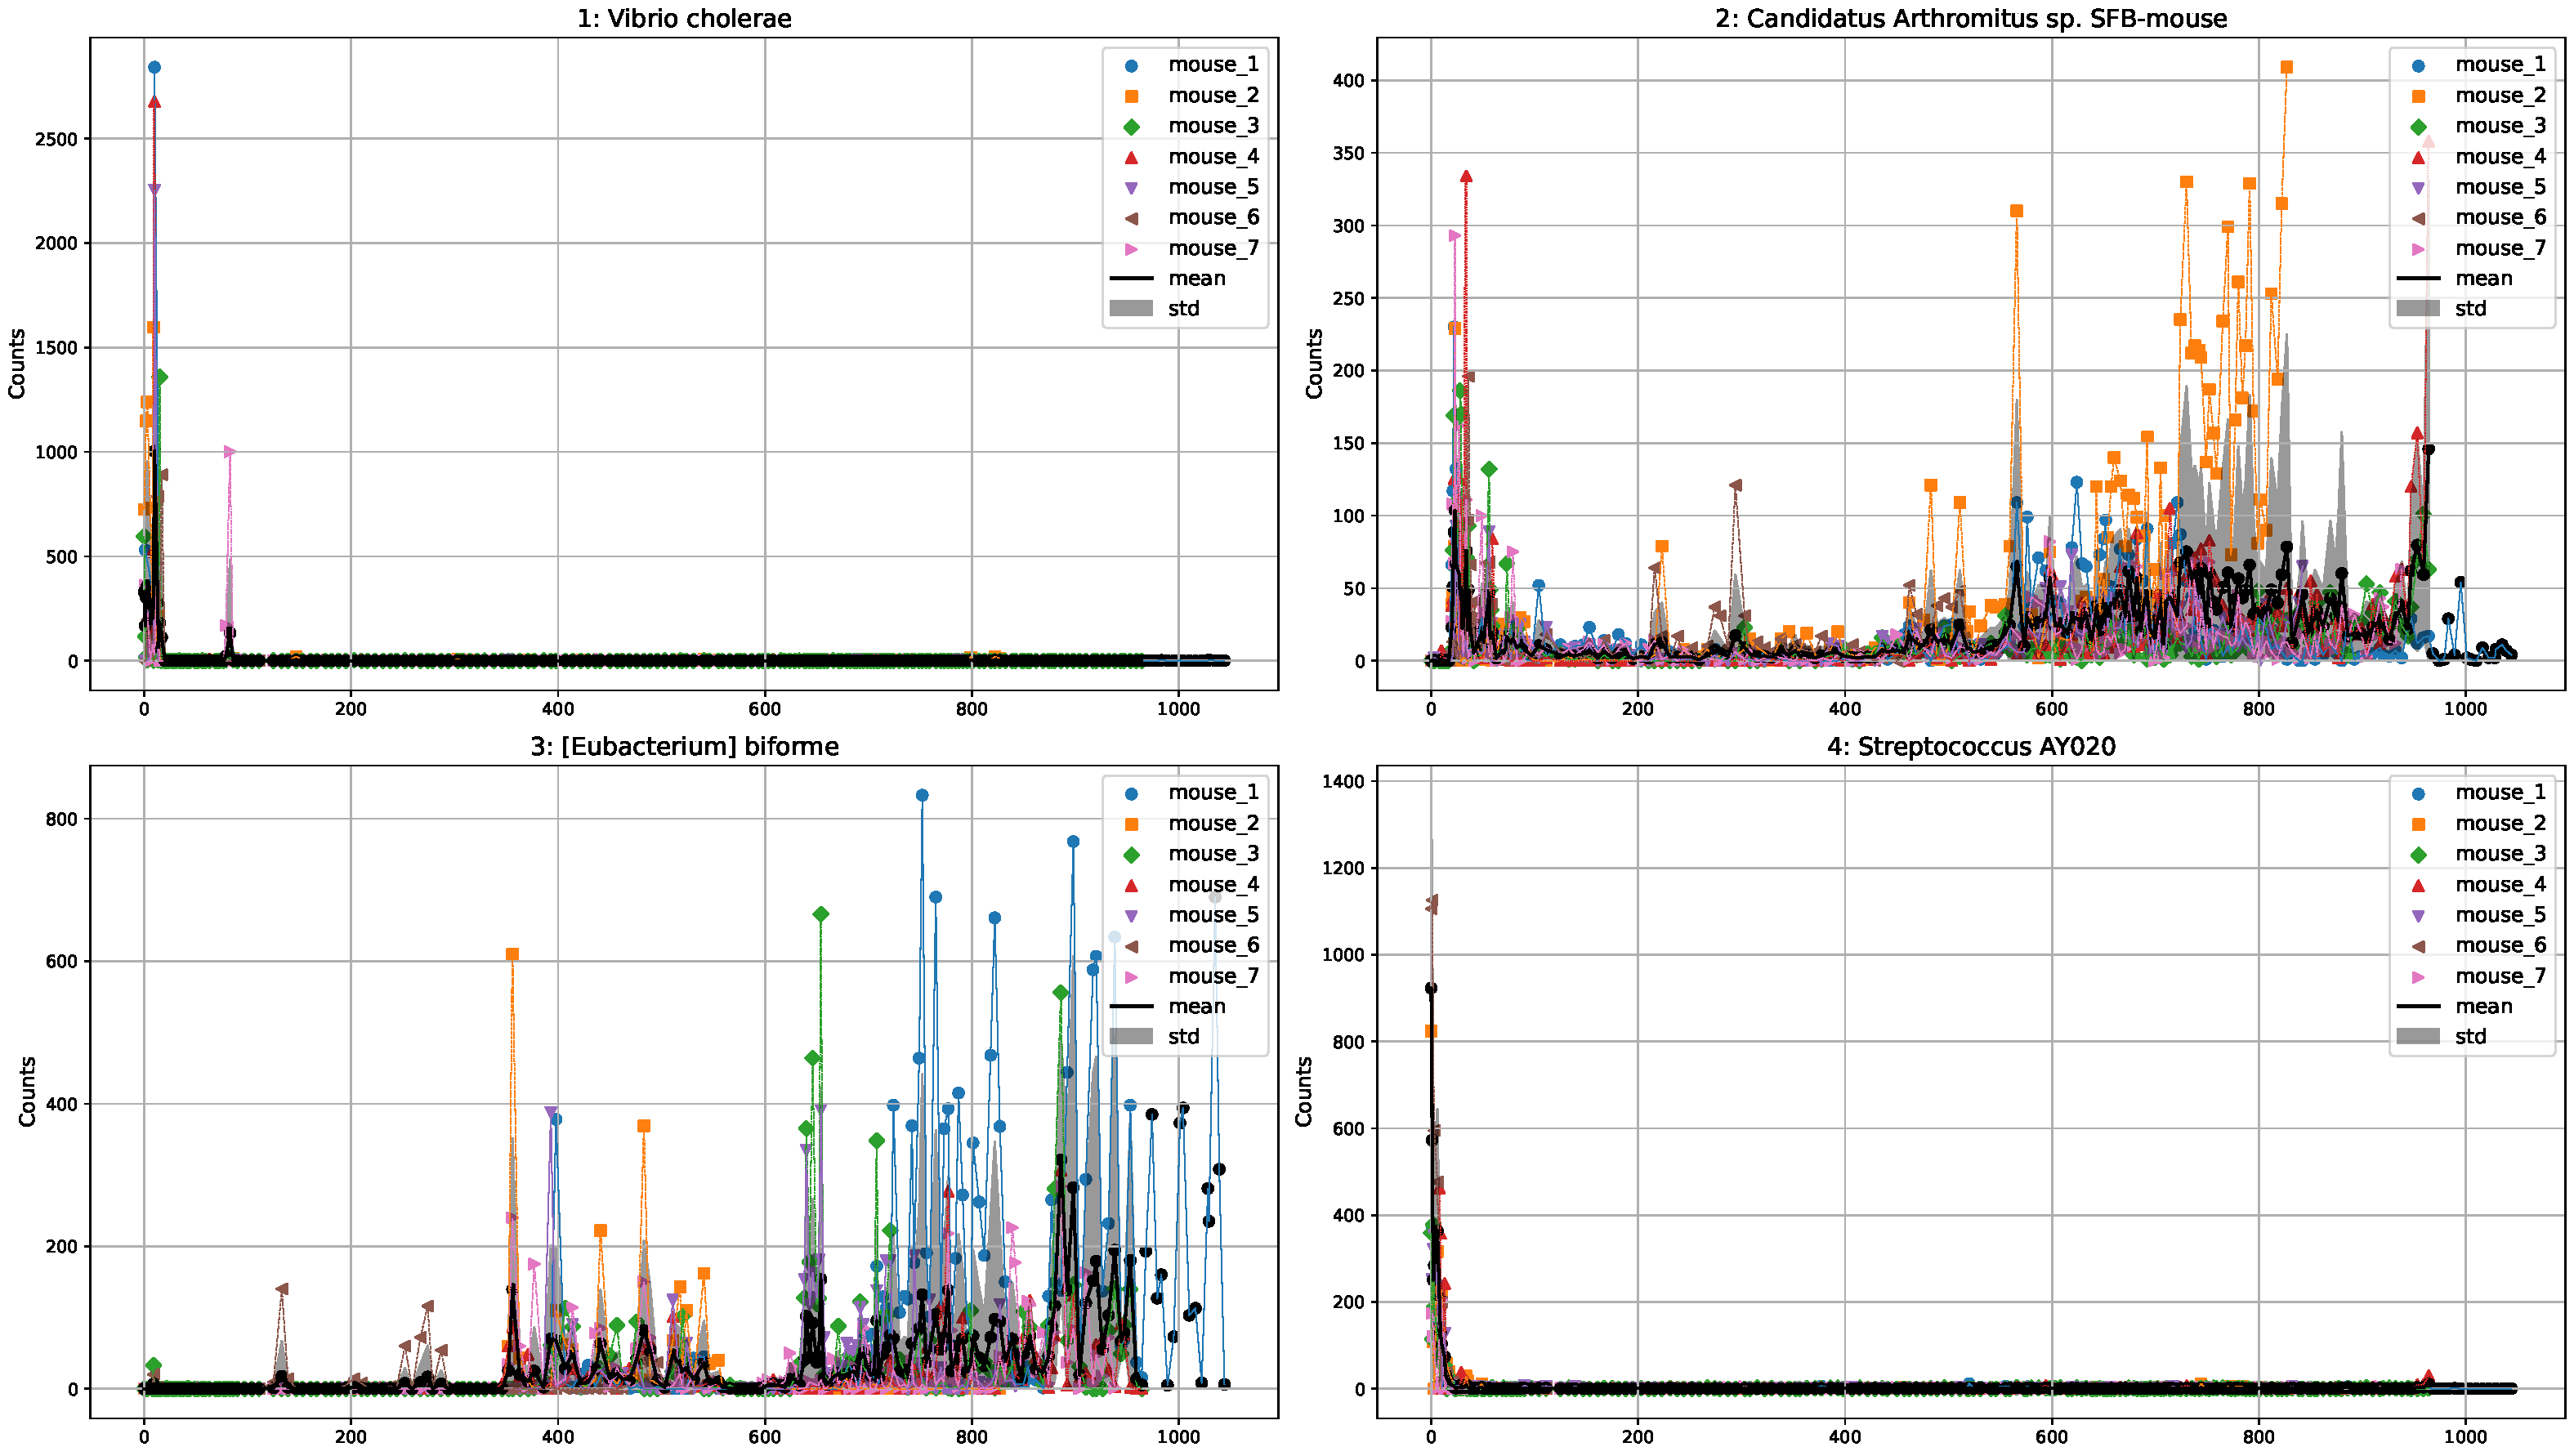
\includegraphics[width=\linewidth]{tables/chapter_2/rare_mean_species.pdf}
    \caption{Caption}
    \label{fig:rare_species}
\end{figure}
\newpage
\section{Gallery of timeseries plots.}



\chapter{Inference through forward linear regression}
Let us suppose that the observed data are produced by an autonomous system of equations of the form, with a multiplicative stochastic noisec term:
\begin{equation*}
    \dot{x}_i = F(x) + x_i\cdot \sigma \cdot \eta_i
\end{equation*}
where the model $f(x)$ is unknown and $\eta_i$ is a normally distributed random variable with zero mean and unit variance. Let us also make the (strong) assumption that the observed data evolves closely to a steady state $x^{*}, f(x^{*}) = 0$. Under the latter assumption, we can linearize the system around the equilibrium:

\begin{equation*}
    \dot{x}_i(t) = J_{F}(x^{*})\cdot (x-x^*) + o(||x- x^*||) + + x_i^*\cdot \sigma \cdot \eta_i
\end{equation*}
the jacobian $J_{F}(x^{*})$ is the so-called community matrix at the equilibrium $x^*$.


This method essentially consists in inferring the $i- th$ row of the community matrix through a least squares regression of the derivative $\dot{x_i}$ (covariate variable) versus the abundances $\{(x_j - x_j^{*})\}_{j=1}^{N}$.
The compositional constraint on the abundances $(\sum_i\, x_i(t) \equiv 1 \,\quad \forall \,t)$, poses a technical difficulty, as the design matrix is singular and hence, the usual least squares regression has no unique solution. To bypass this problem, a forward step regression can be performed instead, which also has the benefit of promoting sparsity. Forward stepwise regression consists in adding one regressor at each step, up to a maximum of $(N-1)$ regressors. By doing this, the columns of the design matrix are always linearly independent. The dataset is first divided into two disjoint subsets: a training dataset and a test dataset. Then, one step of the algorithm works like this:
\begin{enumerate}
    \item For each possible new regressor, the least squares fit is performed on the training dataset
    \item the performance (MSE) of the fits are evaluated on the test dataset
    \item  The new regressor is chosen as the one for which the fit gives the best performance on the test dataset
\end{enumerate}
This basic step is repeated until either the fit improvement falls below a pre-specified threshold, or the maximum number of regressors is reached.

Computational cost can be a concern for this method: in the worst case scenario, the inference of the $i-th$ row requires repeating the least suqares regression $(N-1)$ times. So the overall cost scales as $\sim N^2 \cdot$ cost of one single least squares.

Also, one should account for the error-in-variables problem and the collinearity of the covariate and the regressors.
The covariates $\dot{x_i(t)}$ can be estimated through finite differences:
\begin{equation*}
    \dot{x}_i = \frac{x_i(t+\Delta\,t) - x_i(t)}{\Delta t}
\end{equation*}
or 
\begin{equation*}
    \dot{x}_i = \frac{x_i(t+\Delta\,t) - x_i(t-\Delta t)}{2\,\Delta t} 
\end{equation*}
or higher order formulas.
Clearly, for these numerical estimations to be precise, the time interval $\Delta t$ between consecutive measures needs to be sufficiently small. Otherwise, the data should be interpolated, but this introduces a bias. 


\section{Results with simulated data}

The data 

Una prova su dati simulati che effettivamente evolvono attorno all'equilibri, quindi soltanto per controllare se l'algoritmo funziona come deve. 
La regressione con le derivate inferisce la matrice jacobiana all'equilibrio (community matrix), che per il LV è $J_{i,\,j} = a_{i,j}\cdot \overline{x}_i$, metren la regressione con il modello proposto da fisher inferisce direttamente la matrice delle interazioni, moltiplicata per l'intervallo tra due misure consecutive: $a_{i,j}\cdot \Delta_t$. 
\begin{figure}[H]
    \centering
    \subfigure[]{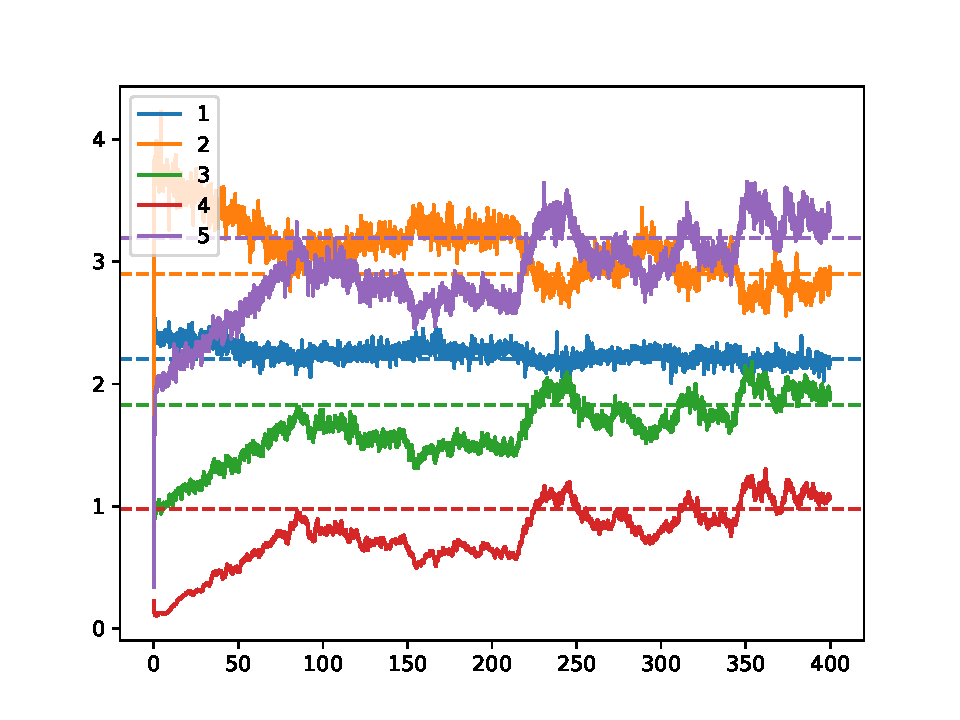
\includegraphics[width=0.7\linewidth]{figures/chapter_3/regression/timeseries_2024-08-24_17-29-06.pdf}}
    \subfigure[]{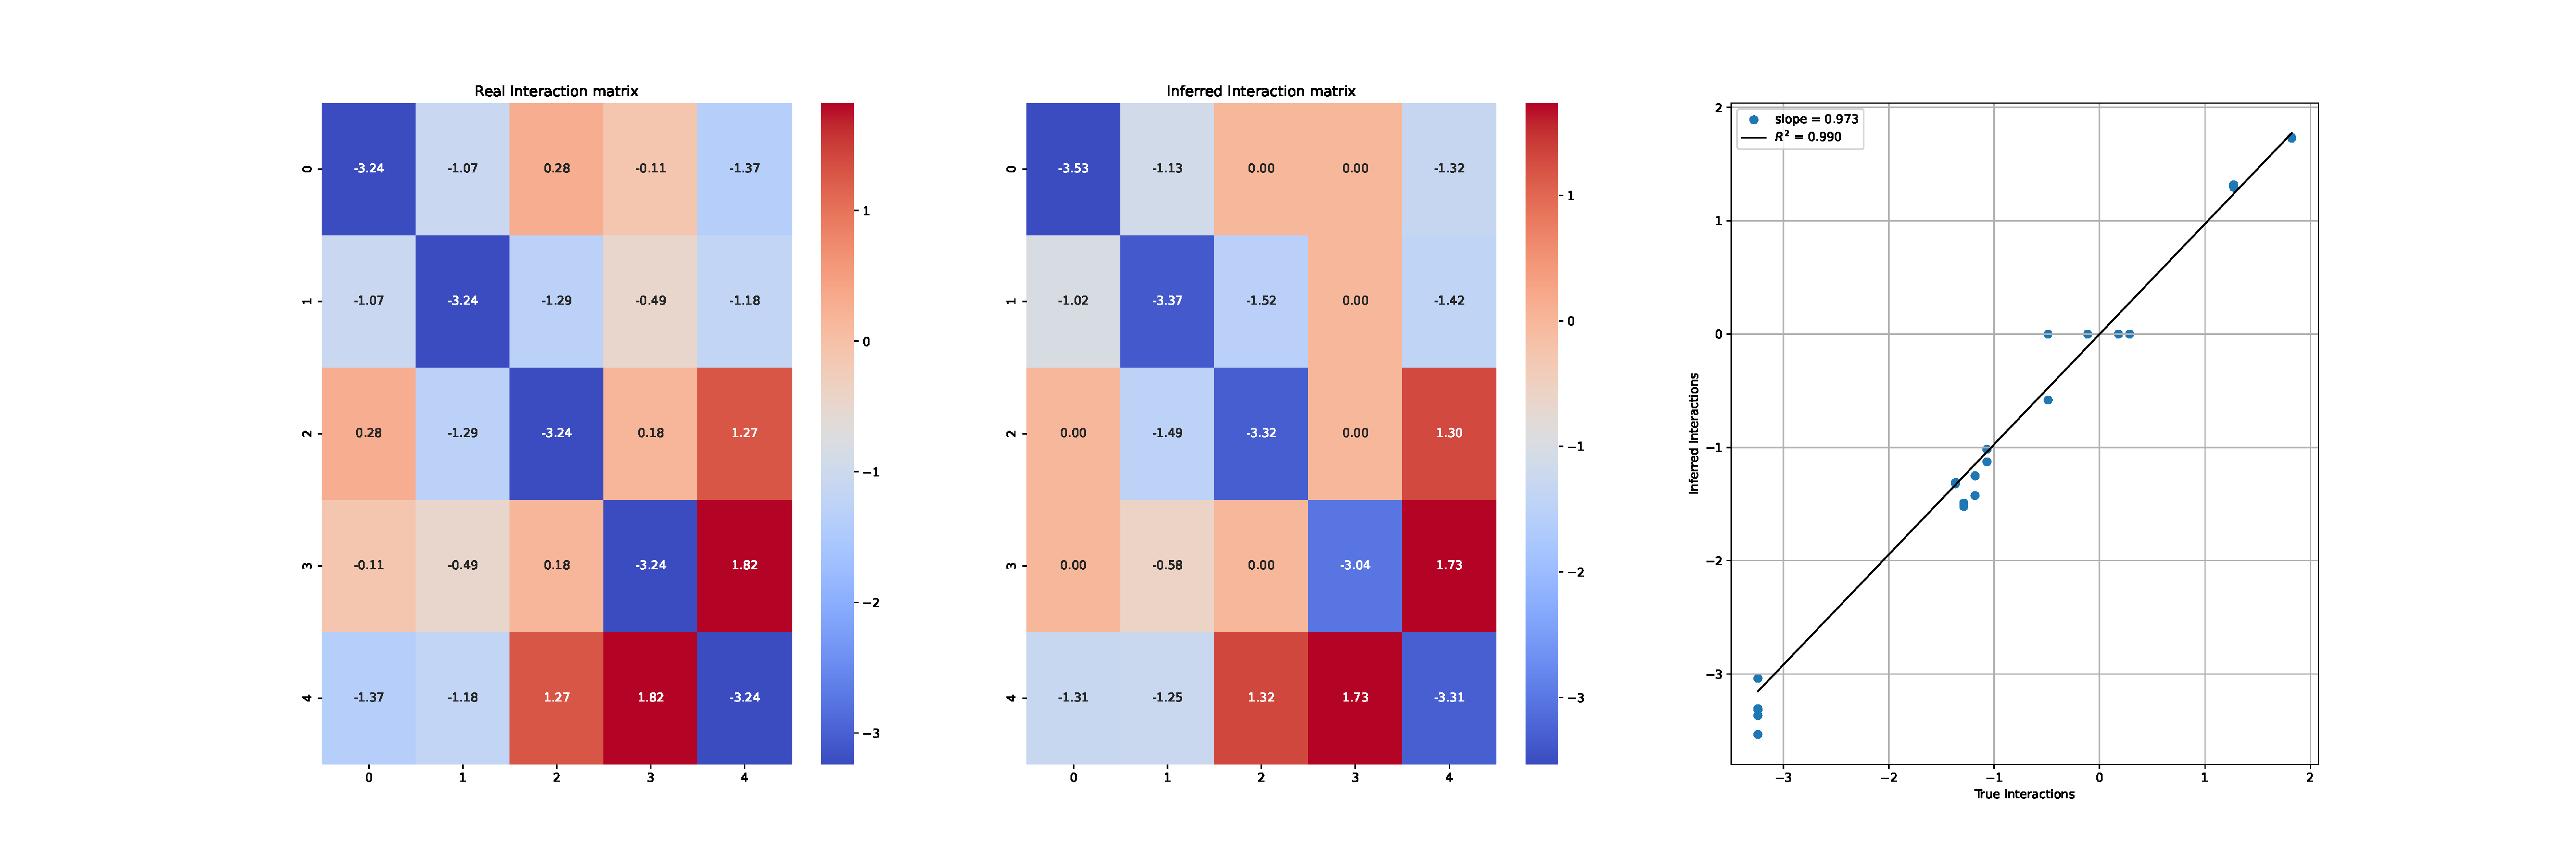
\includegraphics[width=\linewidth]{figures/chapter_3/regression/matrix_comparison_2024-08-24_17-31-23.pdf}}
    \subfigure[]{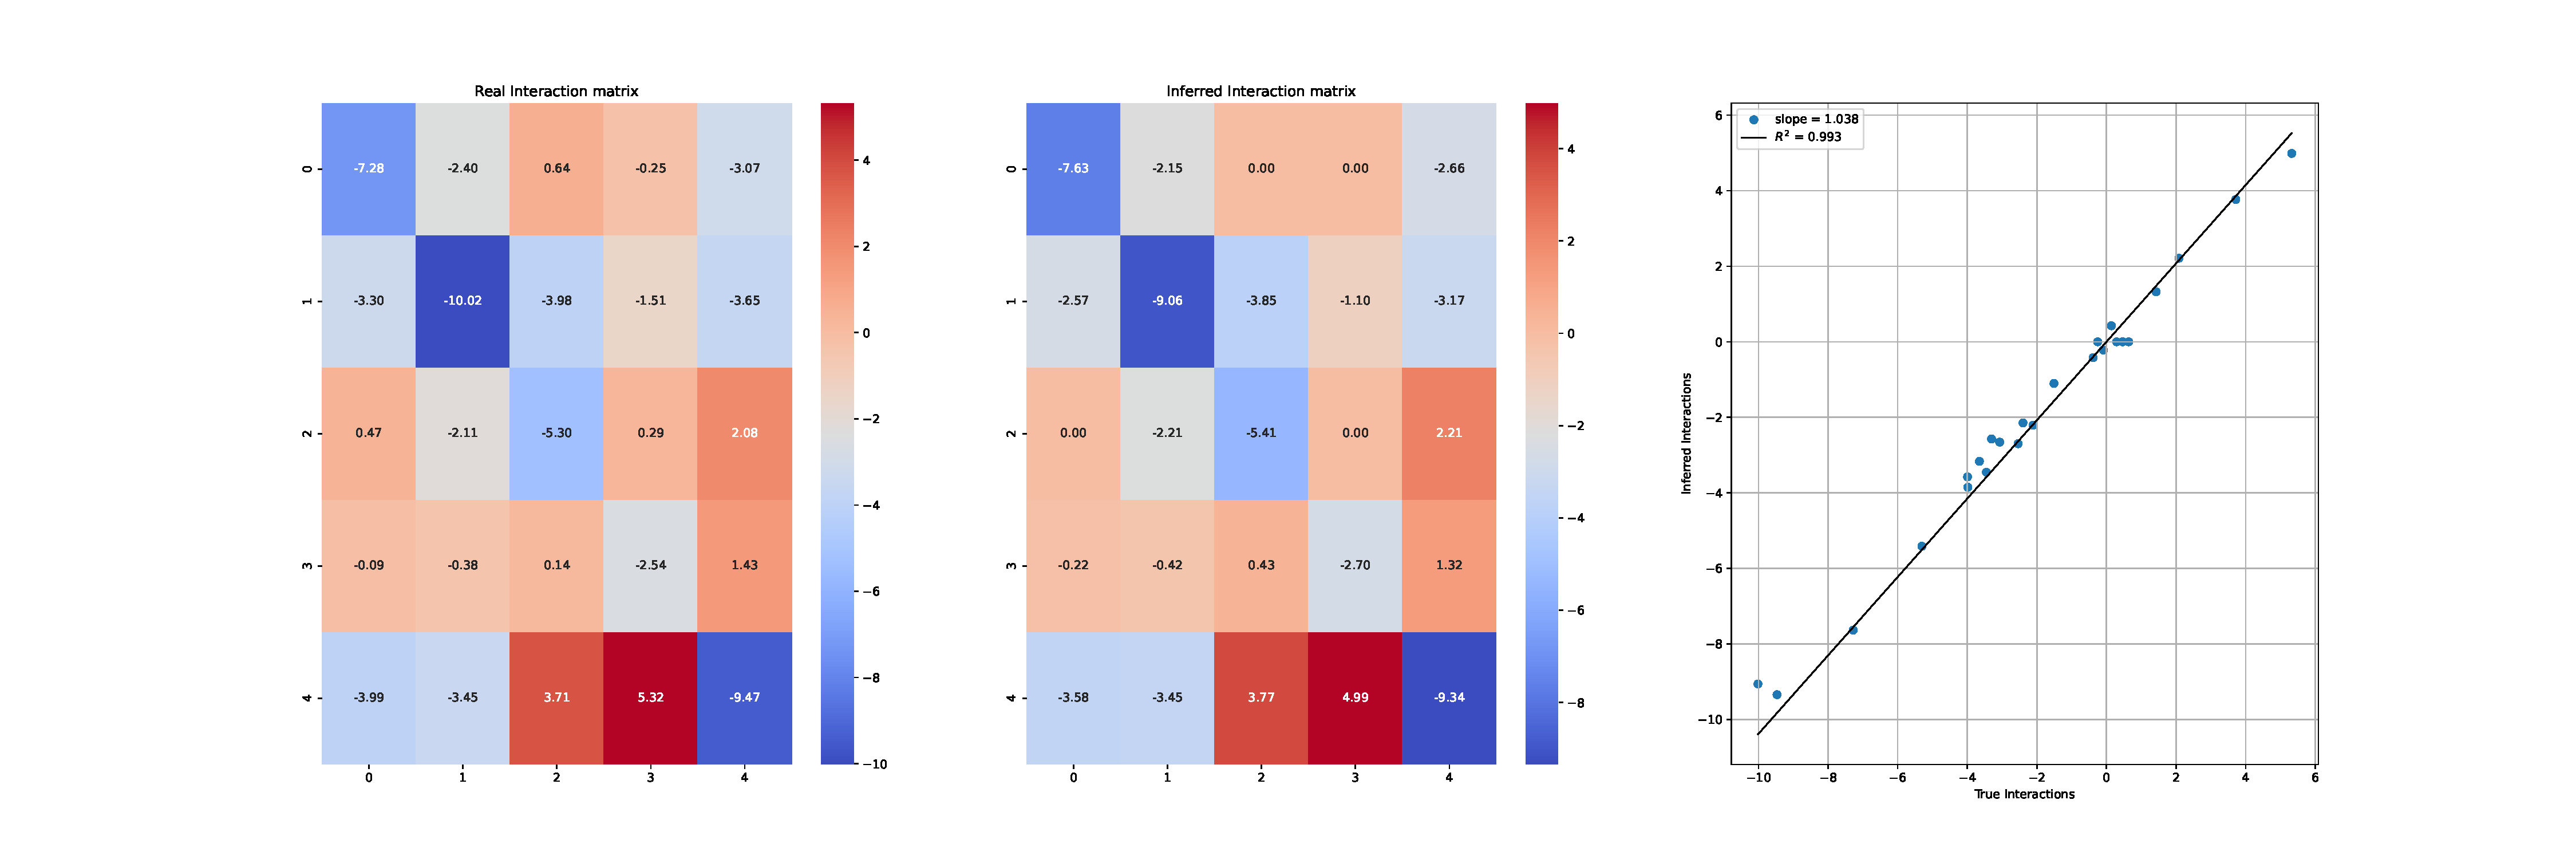
\includegraphics[width=\linewidth]{figures/chapter_3/regression/matrix_comparison_2024-08-24_17-31-24.pdf}}
    \caption{Fig (a): Qui ci sono $5$ specie, giorni $400$, sampling rate $100$ misure al giorno, $sigma=5$. Soglia impostata a $0.1\%$ e numbero di bagging $100$. (Fig. b) metodo di fisher, matrice delle interazioni $a_{i,j}$ reale (sx) e inferita (dx), (Fig. c) classica regressione sulle derivate, matrice di comunità $(J_{i,\,j} = a_{i,\,j}\cdot \overline{x}_i)$ reale e inferita. Performance buone e grossomodo paragonabili. Ci mancherebbe! Se non funzionasse nemmeno su questi dati sarebbe completamente inutile.}
    \label{fig:enter-label}
\end{figure}

\section{Results on mice data}

The method proposed in \parencite{fisher} assumes that:
\begin{enumerate}
\item the observed data is well described by a generalized Lokta-Volterra model, with discrete timesteps and a stochastic noise term,
\item in particular, the observed data is a trajectory in the neighbourhood of a \textbf{stable} (locally? globally? not clear from the paper, but not crucial) and \textbf{feasible} equilibrium $\overline{x}$ The equilibrium values $\overline{x_i}$ can be directly inferred from the data by taking the median (\textcolor{orange}{or mean}) of the abundaces.
\end{enumerate}

The discrete stochastic Lokta Volterra equation is the following:

\begin{equation}
\label{eq:Fisher}
x_i(t + \Delta t^{\small update}) = \eta_i(t) \cdot x_i(t) \cdot \exp \left[ \Delta t^{\small update} \sum_{j=1}^{N} C_{ij} \left[ x_j(t) - \bar{x}_j \right] \right]
\end{equation}

$\eta_i(t)$ is a lognormally distributed variable, representing a stochastic noise. The reason why it is assumed lognormal is that when taking the logaritm we get a normally distributed noise $\eta_i(t) \sim \mathcal{N}(0, \sigma).$ \\
\newline
\begin{equation}
\ln\left[x_i(t + \Delta t^{\small update})\right] - \ln\left[x_i(t)\right] = \zeta_i(t) + \Delta t^{\small update} \sum_{j=1}^{N} C_{ij} \left[ x_j(t) - \bar{x}_j \right]
\end{equation}
Equations \ref{eq:Fisher} simplify to:
\begin{equation*}
    \centering
     \dot{x}_i(t) = x_i(t)\cdot \left[\sum_j\, c_{i,\,j}\, \left(x_j- \overline{x}_j\right)\right]
\end{equation*}
in the limit case $\Delta\, t^{(sampling)}\rightarrow 0$ and $\eta_i(t) \equiv 0$. One can recast these equations into the usual Lokta Volterra equations $ \dot{x}_i(t) = x_i(t)\cdot \left[ r_i\, + \sum_j\, a_{i,\,j}\, x_j \right]$, by identifying
\begin{equation*}
     a_{i,\,j} \equiv c_{i,\,j} \quad \text{and} \quad r_i \equiv - \sum_j\, c_{i,\,j}\,\overline{x}_j
\end{equation*}
$[Ax + r]\overline{x} = 0$ is indeed a necessary condition that must be satisfied by  a feasible equilibrium.





\section{Performance evaluation with simulated data}
Parameters of the simulation are: sampling matrix $C$, sampling rate $m$, noise $\sigma$.
In the code, the entries of the interaction matrix are normalized to unity. In all the following simulations, the entries of the interaction matrix, $c_{i,j}$ are normalized to unity. Re-scaling the interactions is perfectly equivalent to rescaling the update interval, keeping the other parameters fixed.
A possibility must be considered that the update time scale of the evolution process is different from the time scale of the sampling, most likely smaller. In fact, the experimental measures might be taken at consecutive steps $\Delta\,t^{\small (sampling)} = m\cdot \Delta\, t^{\small update}$, where $m > 0$ is an integer multiplying $\Delta t$. For example, it might that the data is well described by a gdLV assuming a timescale is in the order of magnitude of hours, while the measurements are only made each few days. In this case, the accuracy of the fit might well be low. A partial solution, in order to still apply the method when $\Delta t^{(\small sampling)} > \Delta t^{(\small update)}$ is to interpolate the missing experimental values in order to obtain a timeseries where $m = 1$. Of course, the more the two timescales differ, the least this approximation will work. Since we do not know the process timescale in advance when approaching data, we shall try by guess and then compare the results. \textcolor{red}{Question for professors:} what is the expected time scale of bacteria reproduction?
\\

One issue arising with relative abundances data is that a value of zero counts is ambiguous: one cannot known if the species is truly absent, or just so low in abundance that it does not apppear in the sample. 

The fact that the covariate in the regression is a logarithm $y_i = log(x_i t +1) - log(x_i t)$ induces the need to discard all the timepoints where there are zero counts. This makes the inference of interactions impractical for species like those plotted in \ref{fig:rare_species}. For this method is hence reasonable to select the most abundant species with respect to the median counts instead of the mean counts.

Thing to check in simulations are:

\begin{enumerate}
    \item performance at variying threshold on fit improvement,
    \item performance at varying species number $N$,
    \item performance at varying stochasticity level $\sigma$
\end{enumerate}



\begin{figure}[H]
\centering
\subfigure[]{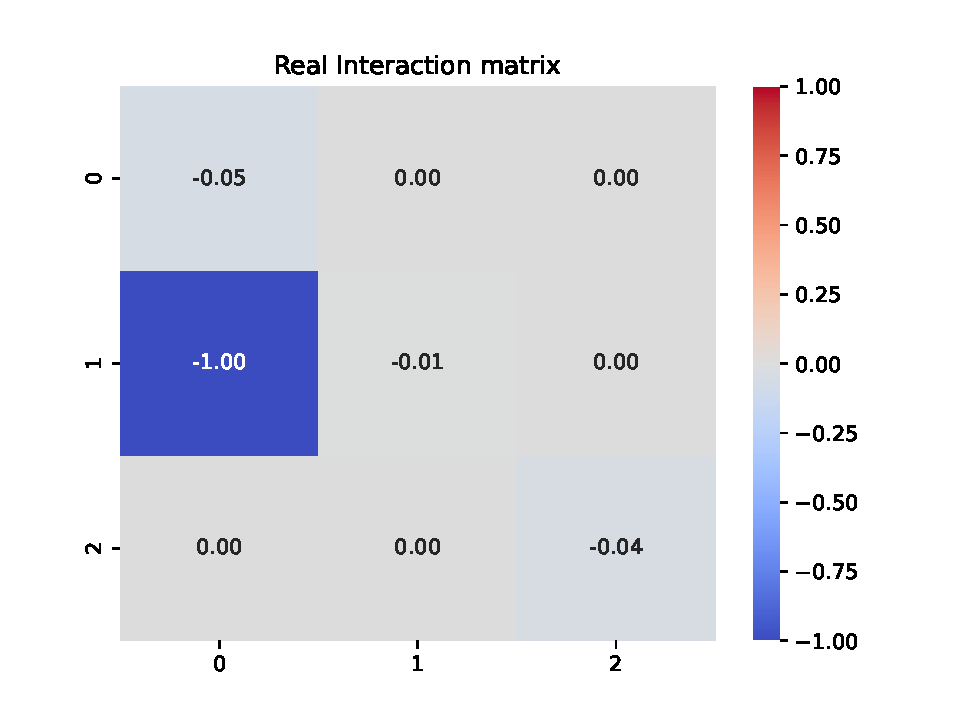
\includegraphics[width = 0.25\linewidth]{figures/chapter_3/matrix_3.pdf}}
\hfill
\subfigure[]{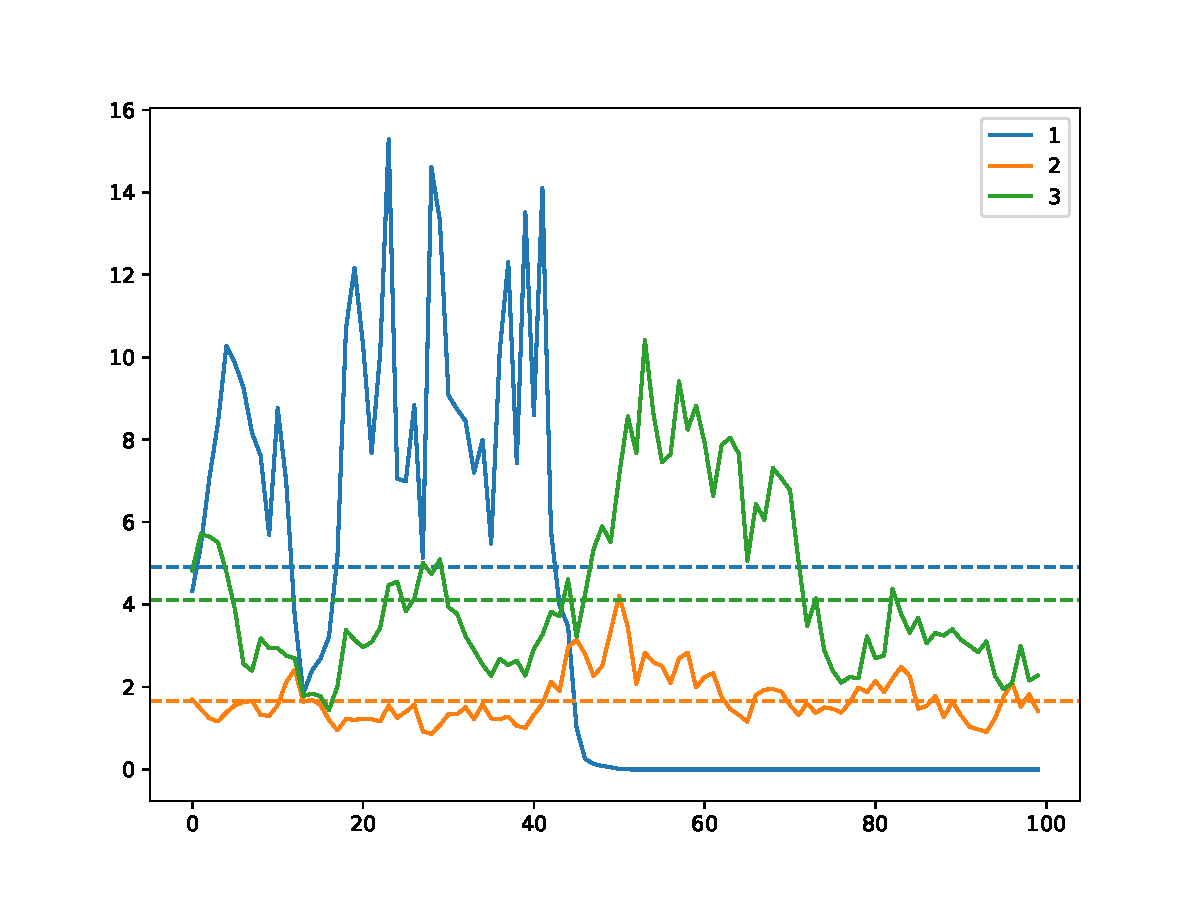
\includegraphics[width = 0.35\linewidth]{figures/chapter_3/discreteTS_species_3_noise_0.2_iter_1.pdf}}
\hfill
\subfigure[]{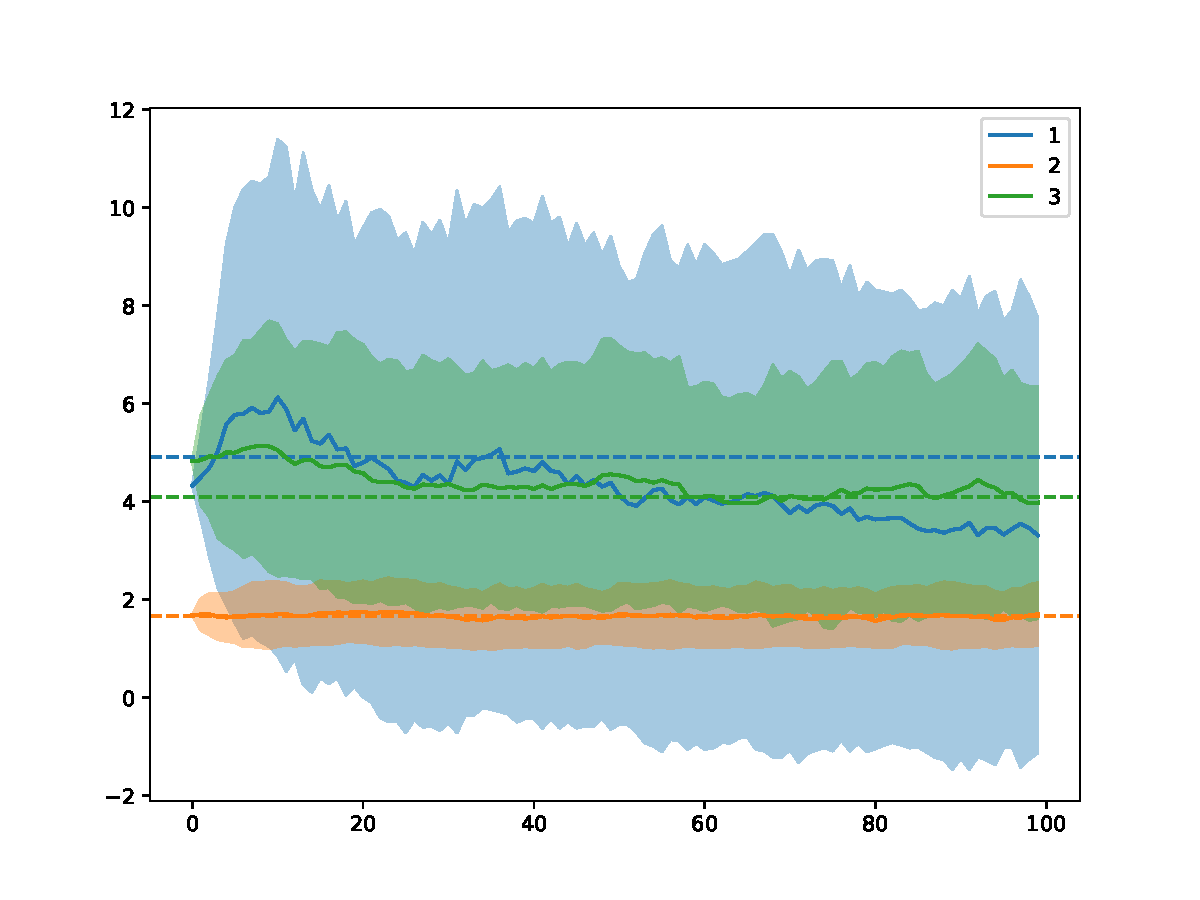
\includegraphics[width = 0.35\linewidth]{figures/chapter_3/discreteTS_species_3_noise_0.2_iter_200.pdf}}
\caption{Parameters are $\sigma = 0.2$. The figure (c) is the mean and std deviation of process repeated $200$ times with fixed initiali conditions. Figure (b) is a typical realization of the process. }
\end{figure}



\section{Results on mice data}
\chapter{Bayesian inference via the Ising Model}

For rare species, i.e. those with abundances below the sampling threshold, we cannot hope to use a model like the Lokta Volterra, simply because we do not have the necessary data. However, from how little we know, we cannot exclude that a species, however low in abundance, can excert a big influence on other species in the ecosystem and prove, indeed, of key global importance.
This is why investigation of the interactions among the pletora of rare species in the ecosystem is equally important.

The supplementary issue arising in this case is that the quality of our data is much worse. In fact, unless improvements in the experimental accuracy, the data we can hope for is only binary: presence/absence. 

An inferential approach of the kind showed in \ref{ch:2} cannot be applied. Here, instead, we try to employ a framework based upon Bayesian Inference that was developed recently \cite{peixoto_MDL}. The key assumption of this scheme is that the time series of binary data is well described by assuming an Ising model. However, this is only the simplest option. Indeed, the framework developed by the author is much more general and could be extended in future work to other cases as well.

Will the interactions obtained with this kind of data be coherent with those obtained through the LV? Most probably not, but for now we just make preliminary tentatives.



\printbibliography


\backmatter
\end{document}







